% Het document is een boek op A4 papier in recto te printen.
\documentclass[a4paper,10pt,oneside]{book}

% Babel zorgt ervoor dat titels en dergelijke in de juiste taal te voorschijn komen
\usepackage[dutch]{babel}

% Zorgt ervoor dat karakters met accenten ingevoerd kunnen worden, zoals é.
\usepackage[utf8]{inputenc}
% Zorgt voor correcte output van karakters met accenten
\usepackage[T1]{fontenc}
% Font met T1 ondersteuning.
\usepackage{lmodern}

% De ams packages zorgen voor alle wiskundige zaken.
\usepackage{amsmath}
\usepackage{amsfonts}
\usepackage{amssymb}
\usepackage{amsthm}

% Subfiles zorgt ervoor dat we het bestand kunnen onderverdelen en elk deel apart kunnen compileren.
\usepackage{subfiles}

% Enumerate zorgt voor mooiere enumerates
\usepackage{enumerate}

% Hyperref zorgt voor clickable stuff.
\usepackage{hyperref} 

% Float zorgt ervoor dat we figuren op de juiste plaats in de tekst kunnen zetten.
\usepackage{float}

% Url zorgt voor urls, duh...
\usepackage{url}

% Pdfpages zorgt ervoor dat we .pdf bestanden kunnen toevoegen.
\usepackage[final]{pdfpages}

% Footnote zorgt voor mooie footnotes.
\usepackage{footnote}

% Tikz is voor de tekeningen (diagrammen).
\usepackage{tikz}
\usetikzlibrary{topaths,calc}

% Mdframed zorgt voor kaders.
\usepackage{mdframed}

% Float zorgt ervoor dat je figuren op de juiste plaats kan zetten.
\usepackage{float}

\setlength{\textwidth}{6in} 
\addtolength{\hoffset}{-0.5in}
\setlength{\topmargin}{-0.2in}
\setlength{\textheight}{9in}

\makeatletter
\renewcommand*\env@matrix[1][*\c@MaxMatrixCols c]{%
  \hskip -\arraycolsep
  \let\@ifnextchar\new@ifnextchar
  \array{#1}}
\makeatother

\begin{document}


\begin{titlepage}
\hbox{
\hspace*{0.2\textwidth}
\rule{1pt}{\textheight}
\rule{2pt}{\textheight}
\rule{3pt}{\textheight}
\rule{4pt}{\textheight}
\rule{5pt}{\textheight}
\hspace*{0.05\textwidth}
\parbox[b]{0.75\textwidth}
{
{\noindent\Huge\bfseries Lineaire Algebra}\\[2\baselineskip]

{\huge \textsc{Tom Sydney Kerckhove}}\\\\\\
{Met dank aan}\\\\
{\Large \textsc{Ward Schodts}}\\\\
{\large \textsc{Frederik Goovaerts}}\\
{\large \textsc{Willem Van Onsem}}\\
{\large \textsc{Nicholas Haesen}}\\
{\large \textsc{Thomas Dierckx}}\\
{\large \textsc{Jorik De Waen}}\\
{\large \textsc{Egon Okerman}}\\
{\large \textsc{Giel Dops}}\\
{\textsc{Tijl Jappens}}\\
{\textsc{Jari Peeperkorn}}\\
{\textsc{Haroen Viaene}}\\
{\textsc{Eline Vrijsen}}\\
{\textsc{Thalia Kayma}}\\
{\textsc{Nick Van den Broeck}}\\


{\normalsize Gestart op: 26 september 2013}\\
{\normalsize Gecompileerd op: \today}\\

{\small Versie 1.0.1.0}



\vspace{0.4\textheight} % Whitespace
}
}
\end{titlepage}

\subfile{extra/voorwoord}

\newpage
\tableofcontents
\pagebreak

\subfile{extra/inleiding}

\part{Theorie}
\subfile{oplossingen/hoofdstukken/hoofdstuk_1_theorie}
\subfile{oplossingen/hoofdstukken/hoofdstuk_2_theorie}
\subfile{oplossingen/hoofdstukken/hoofdstuk_3_theorie}
\subfile{oplossingen/hoofdstukken/hoofdstuk_4_theorie}
\subfile{oplossingen/hoofdstukken/hoofdstuk_5_theorie}
\subfile{oplossingen/hoofdstukken/hoofdstuk_6_theorie}

\part{Oefeningen}
\subfile{oplossingen/hoofdstukken/hoofdstuk_1_oefeningen}
\subfile{oplossingen/hoofdstukken/hoofdstuk_2_oefeningen}
\subfile{oplossingen/hoofdstukken/hoofdstuk_3_oefeningen}
\subfile{oplossingen/hoofdstukken/hoofdstuk_4_oefeningen}
\subfile{oplossingen/hoofdstukken/hoofdstuk_5_oefeningen}
\subfile{oplossingen/hoofdstukken/hoofdstuk_6_oefeningen}

\part{Extra}
\subfile{extra/notatie}
\subfile{extra/tipsntricks}
\subfile{extra/andere_bewijzen}
\subfile{extra/venn_diagram}

\chapter{Zelfreflecties}
De opgaven voor deze zelfreflecties staan achteraan dit boek.
\subfile{oplossingen/zelfreflecties/zelfreflectie_1}
\subfile{oplossingen/zelfreflecties/zelfreflectie_2}
\subfile{oplossingen/zelfreflecties/zelfreflectie_3}
\subfile{oplossingen/zelfreflecties/zelfreflectie_4}
\subfile{oplossingen/zelfreflecties/zelfreflectie_5}
\subfile{oplossingen/zelfreflecties/zelfreflectie_6}

\chapter{Oude Examens}
De opgaven voor deze examens staan achteraan dit boek.
\subfile{oplossingen/examens/examen_2009_januari}
\subfile{oplossingen/examens/examen_2010_januari}
\subfile{oplossingen/examens/examen_2010_augustus}
\subfile{oplossingen/examens/examen_2011_januari}
\subfile{oplossingen/examens/examen_2012_augustus}

\chapter{Huistaken}
\subfile{oplossingen/huistaken/huistaak_1}
\subfile{oplossingen/huistaken/huistaak_2}

\appendix
\chapter{Errata van de curus}
\subfile{extra/errata}

\chapter{Opgaven}
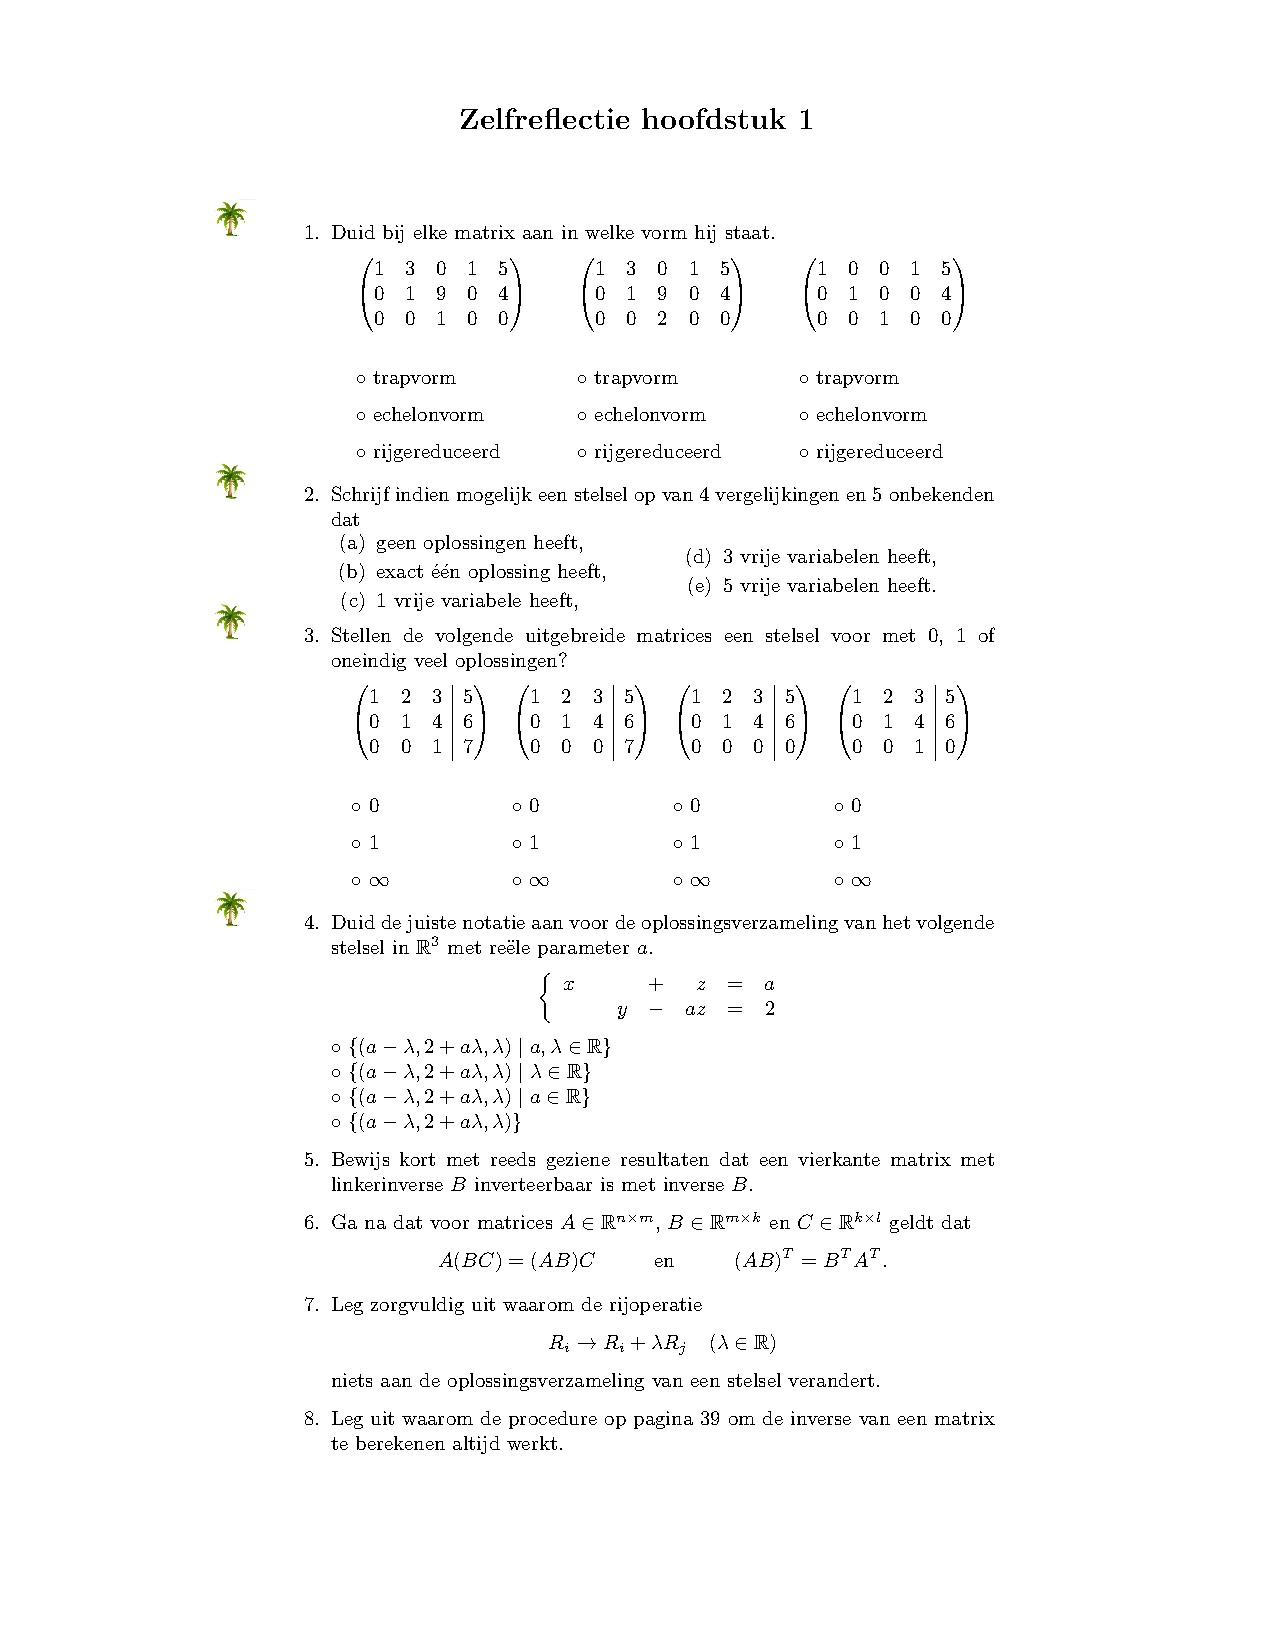
\includepdf[pages=-]{opgaven/zelfreflecties/zelfreflectie_H1.pdf}
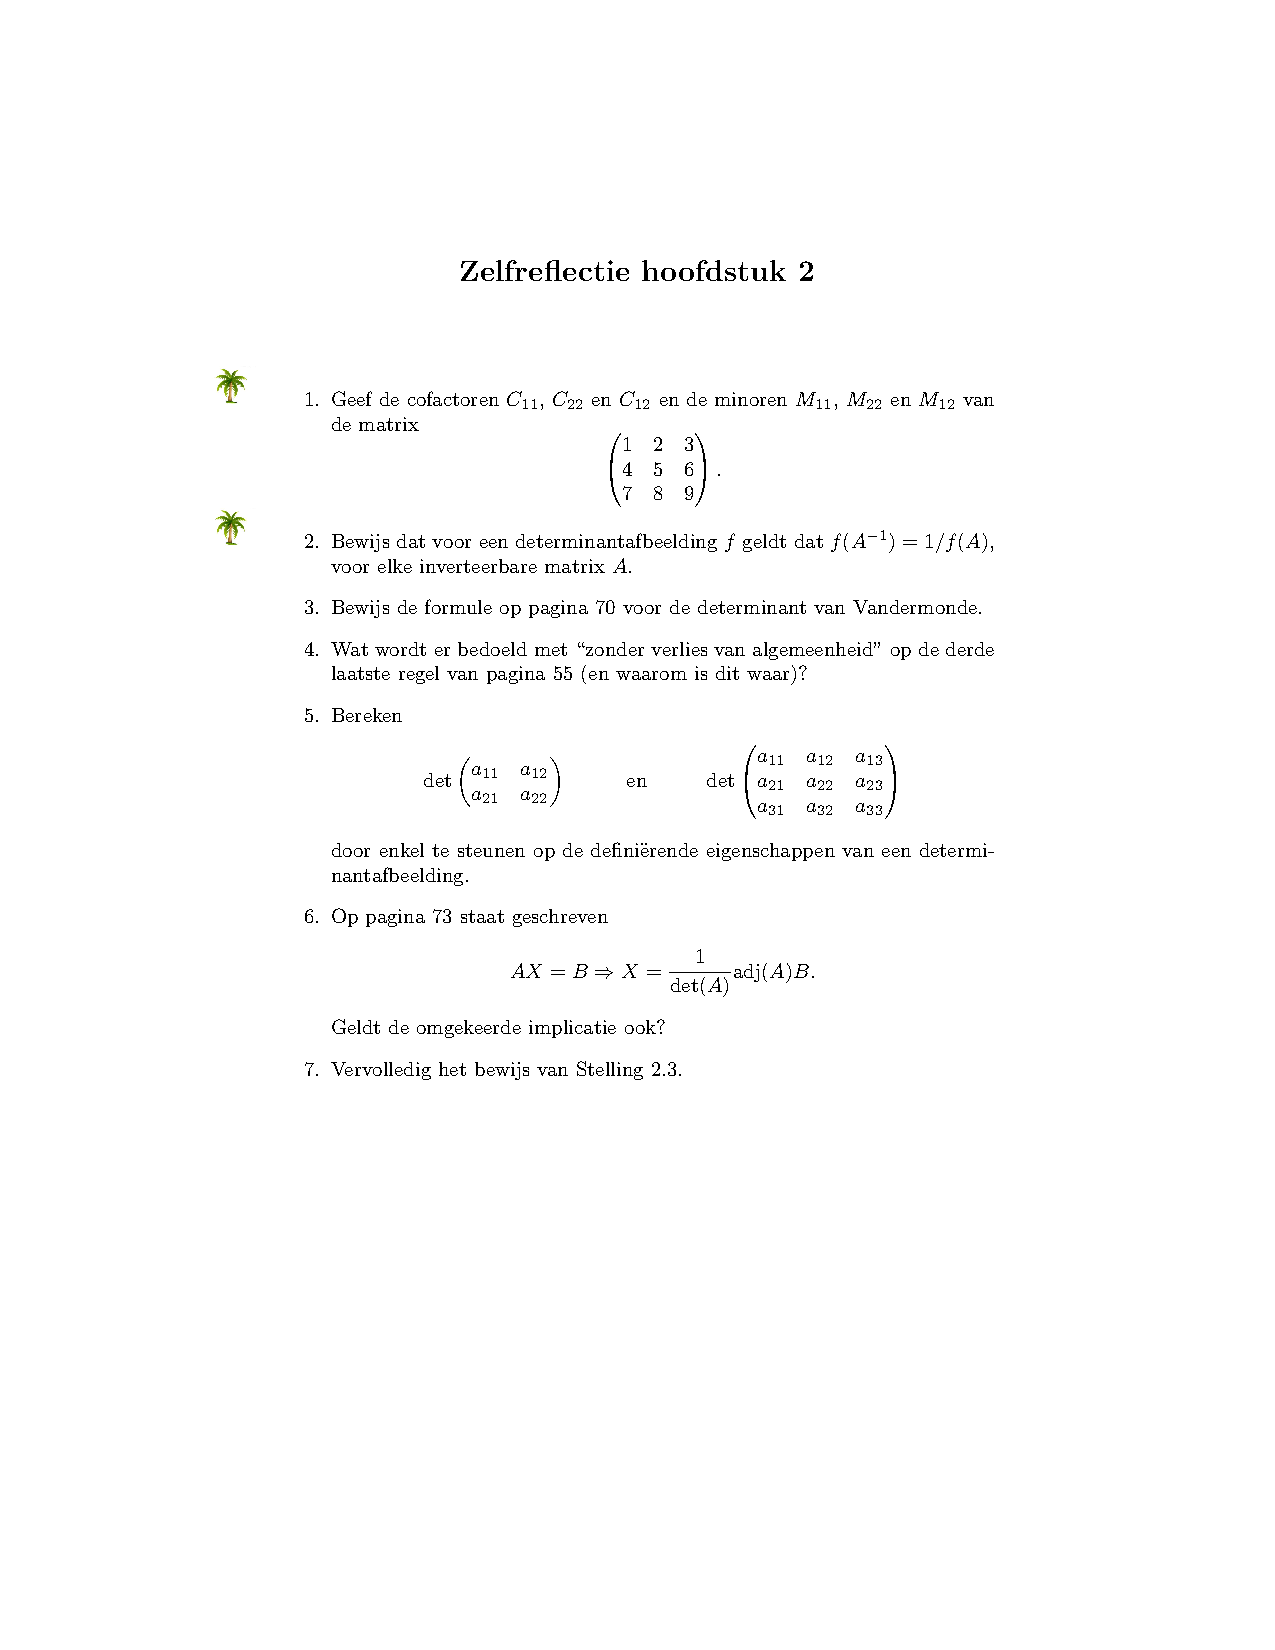
\includepdf[pages=-]{opgaven/zelfreflecties/zelfreflectie_H2.pdf}
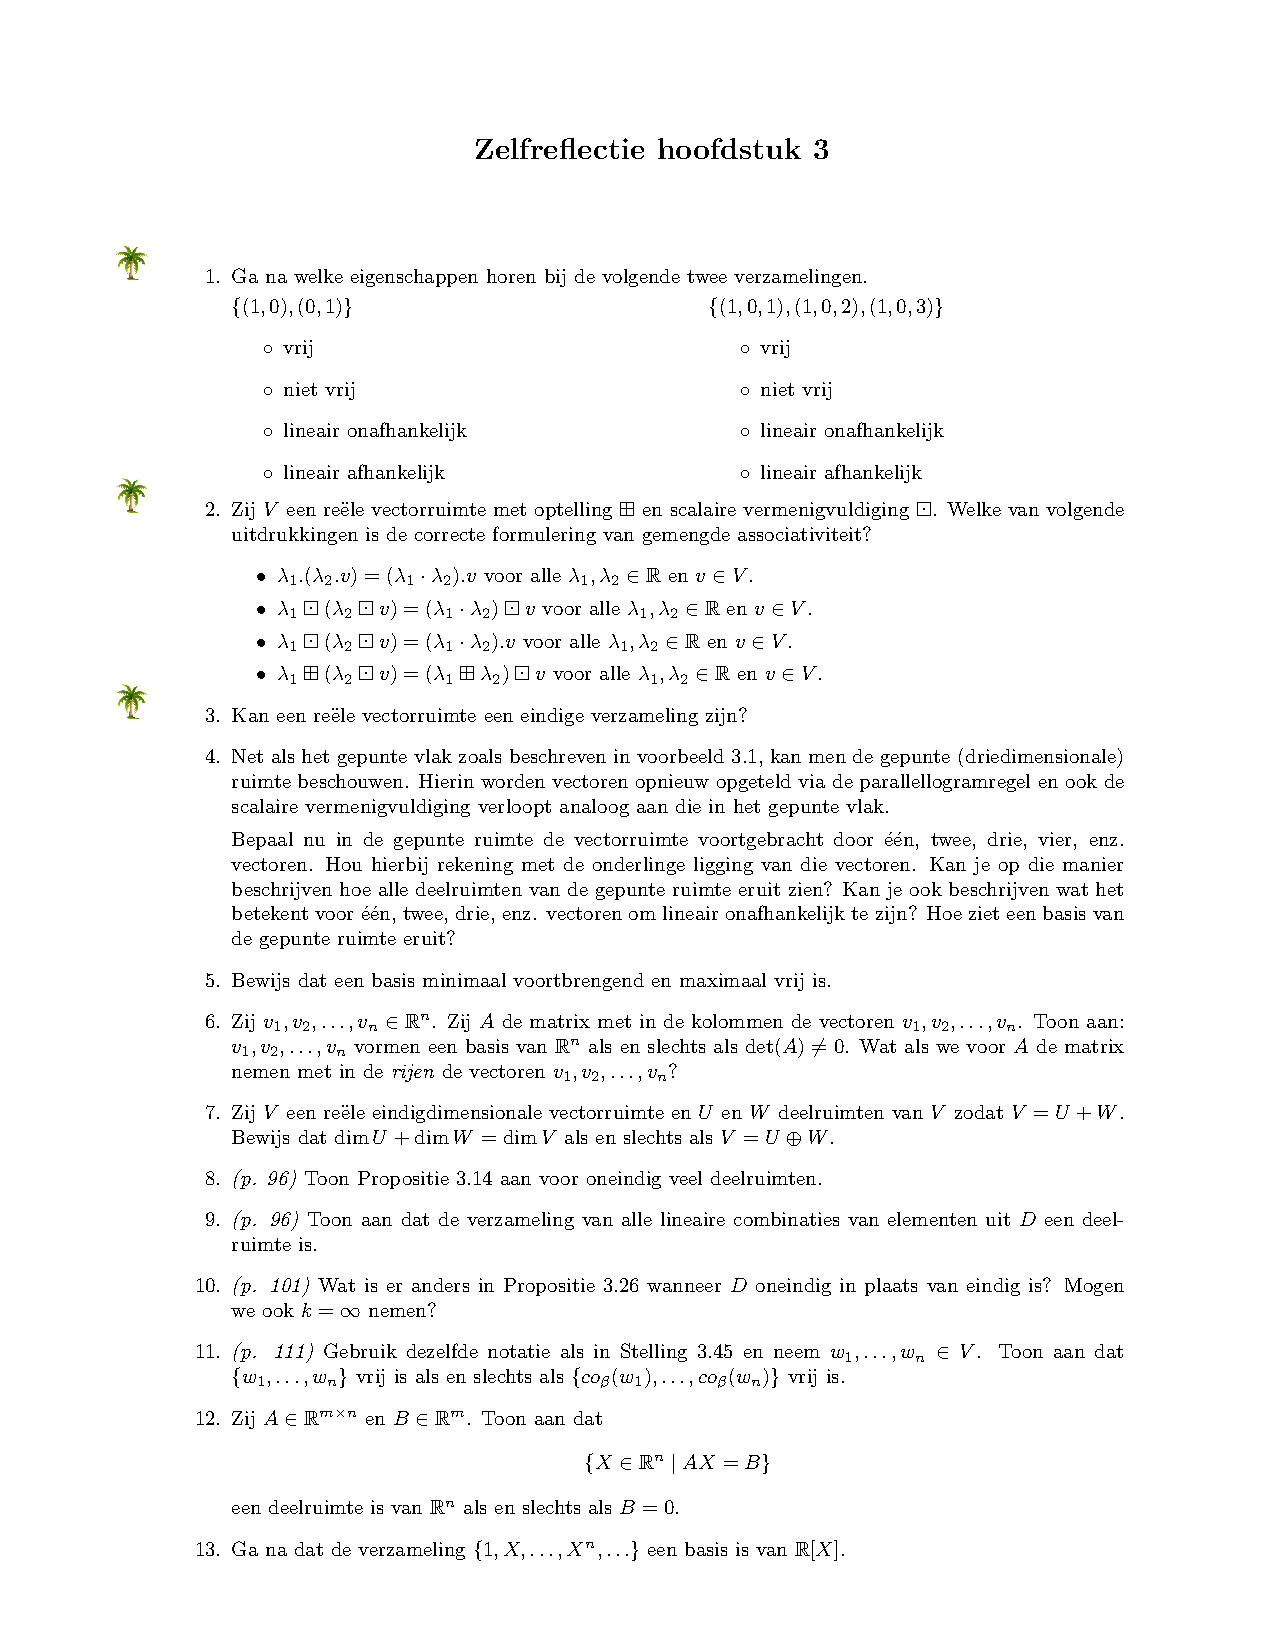
\includepdf[pages=-]{opgaven/zelfreflecties/zelfreflectie_H3.pdf}
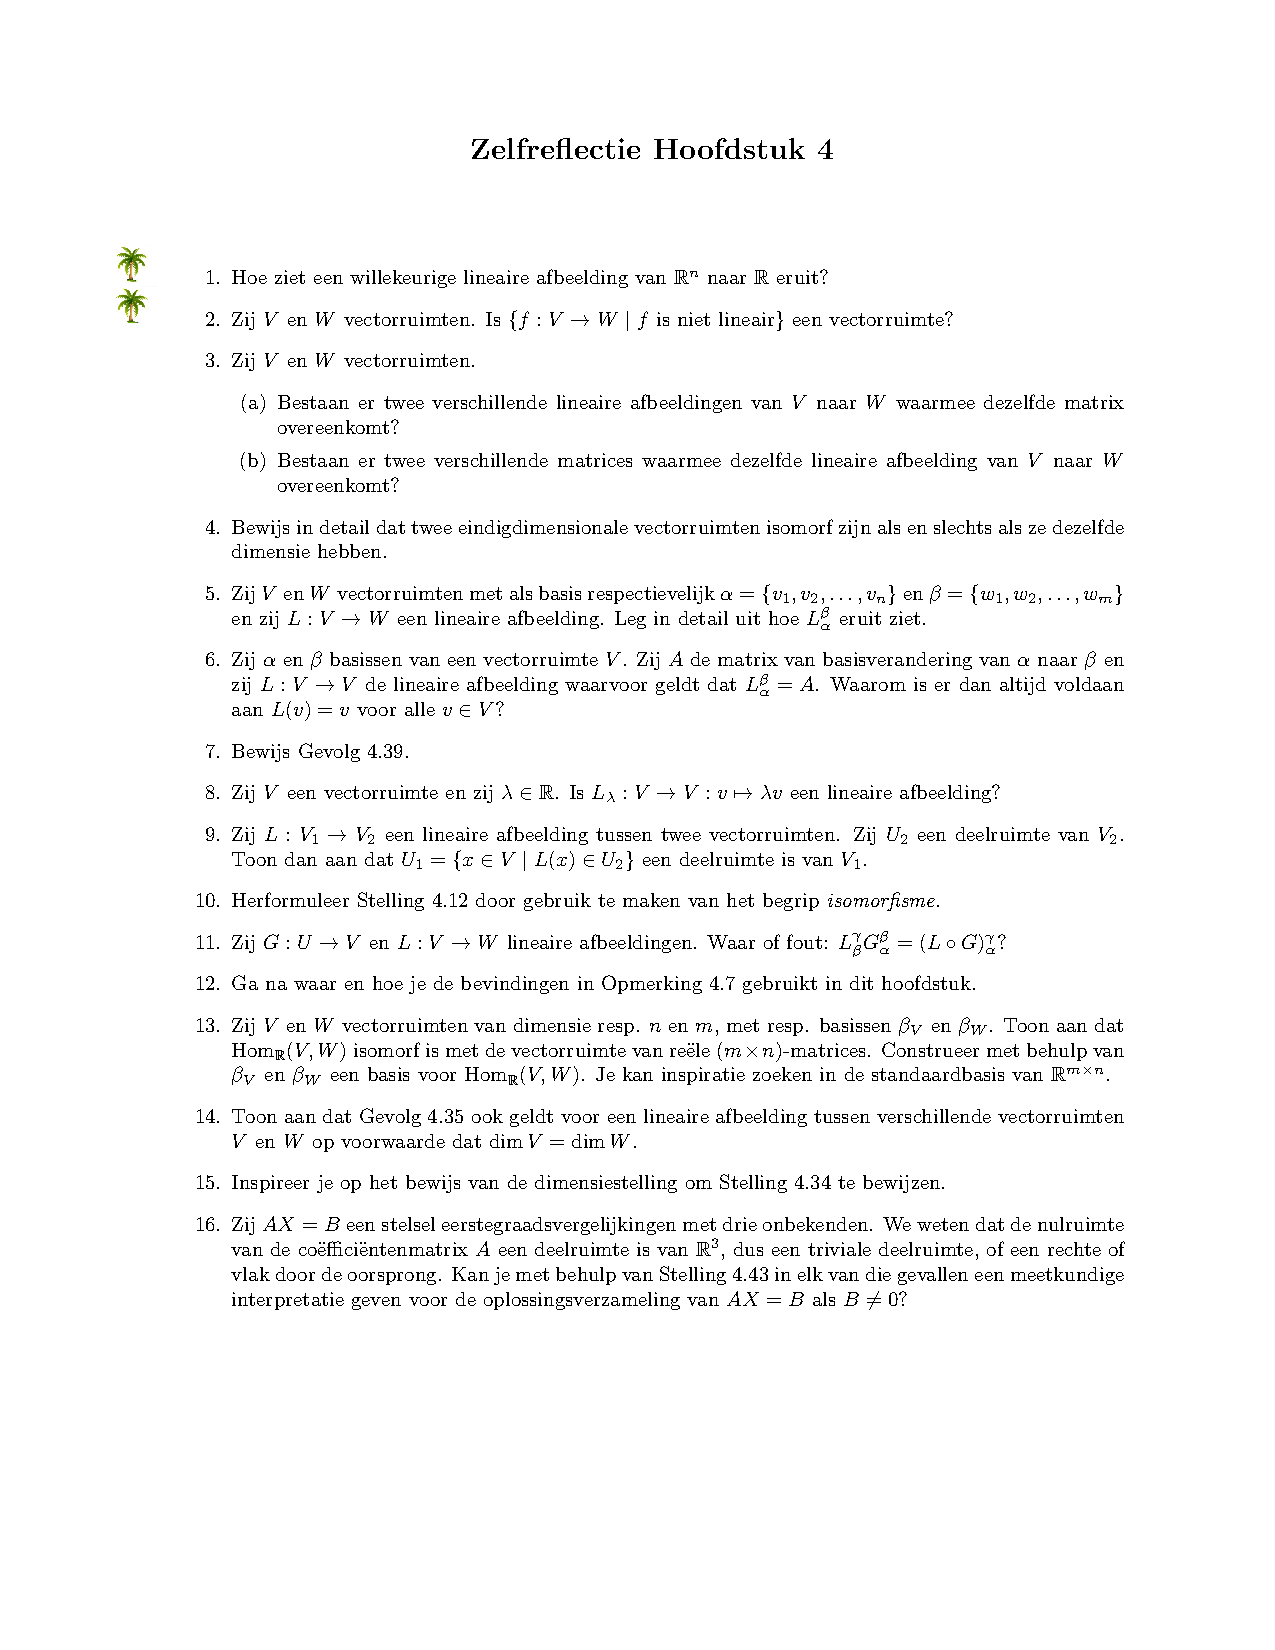
\includepdf[pages=-]{opgaven/zelfreflecties/zelfreflectie_H4.pdf}
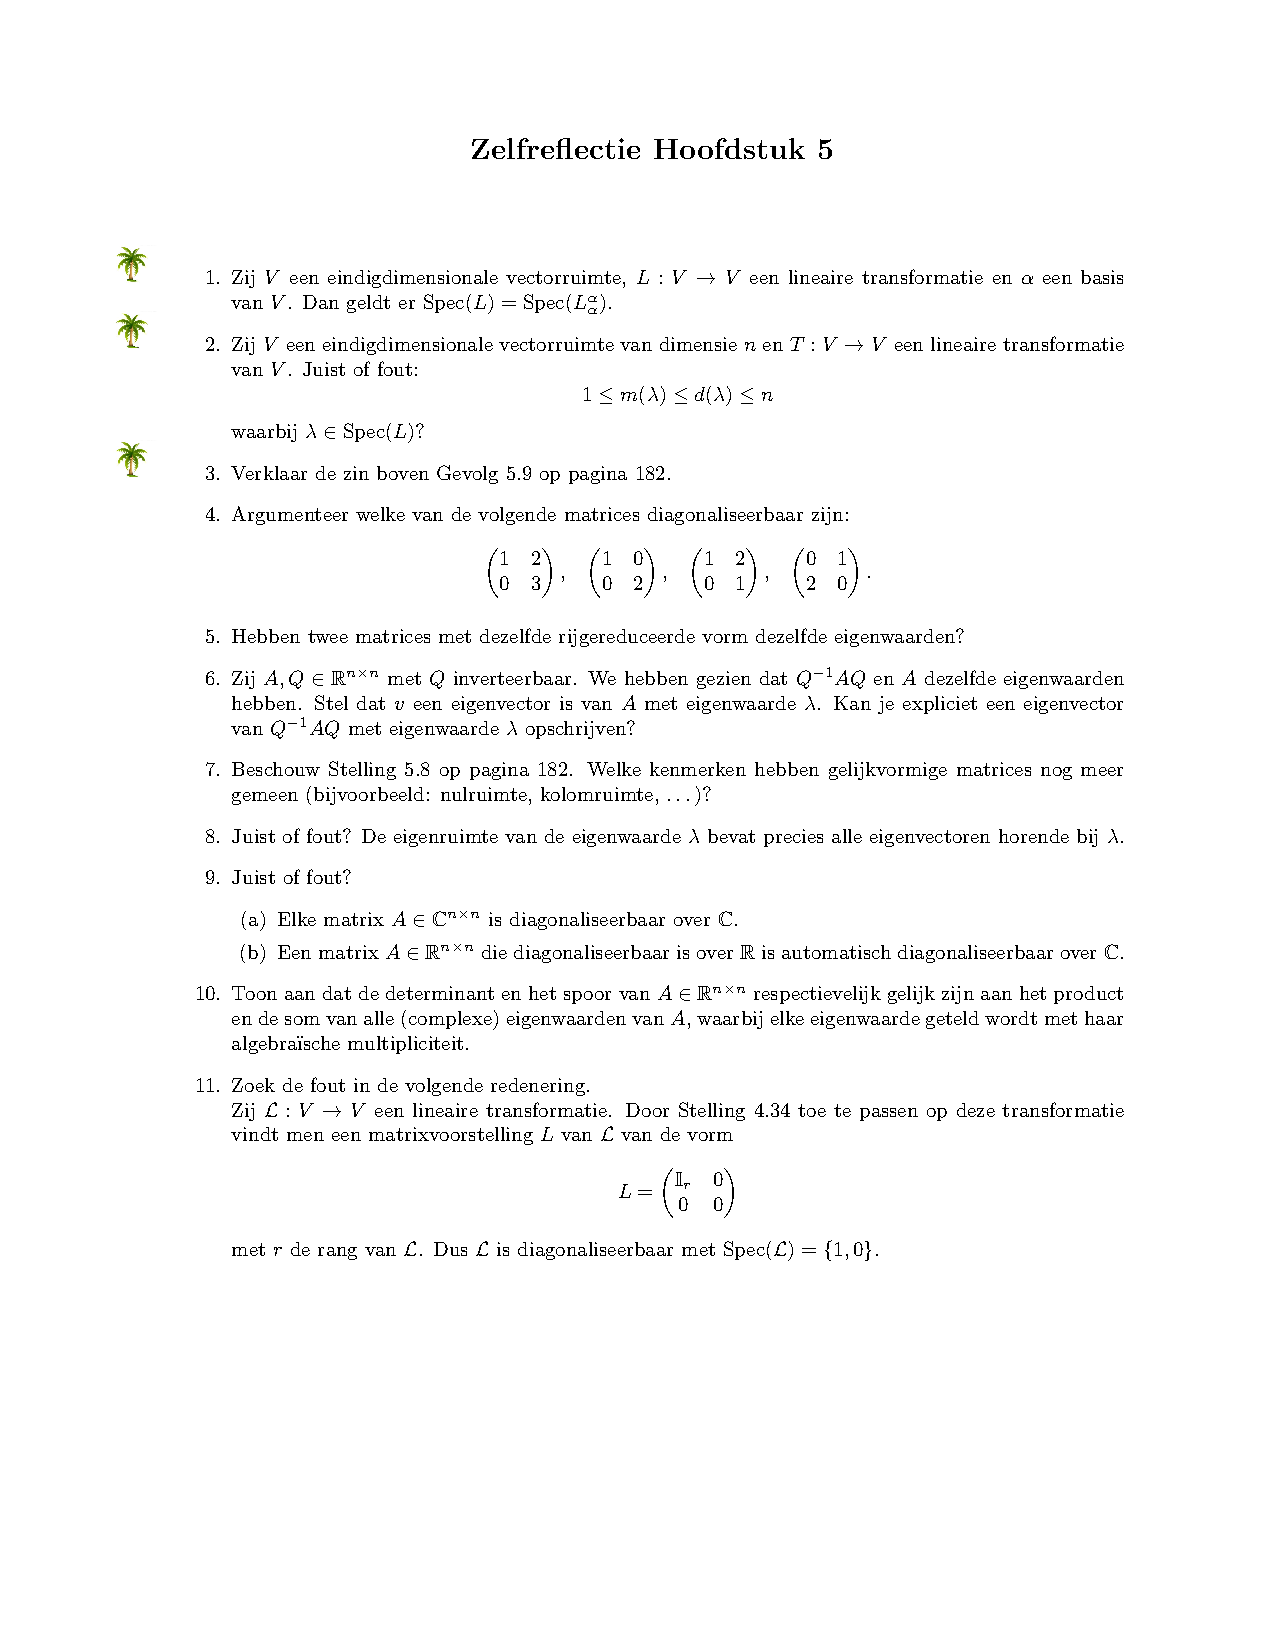
\includepdf[pages=-]{opgaven/zelfreflecties/zelfreflectie_H5.pdf}
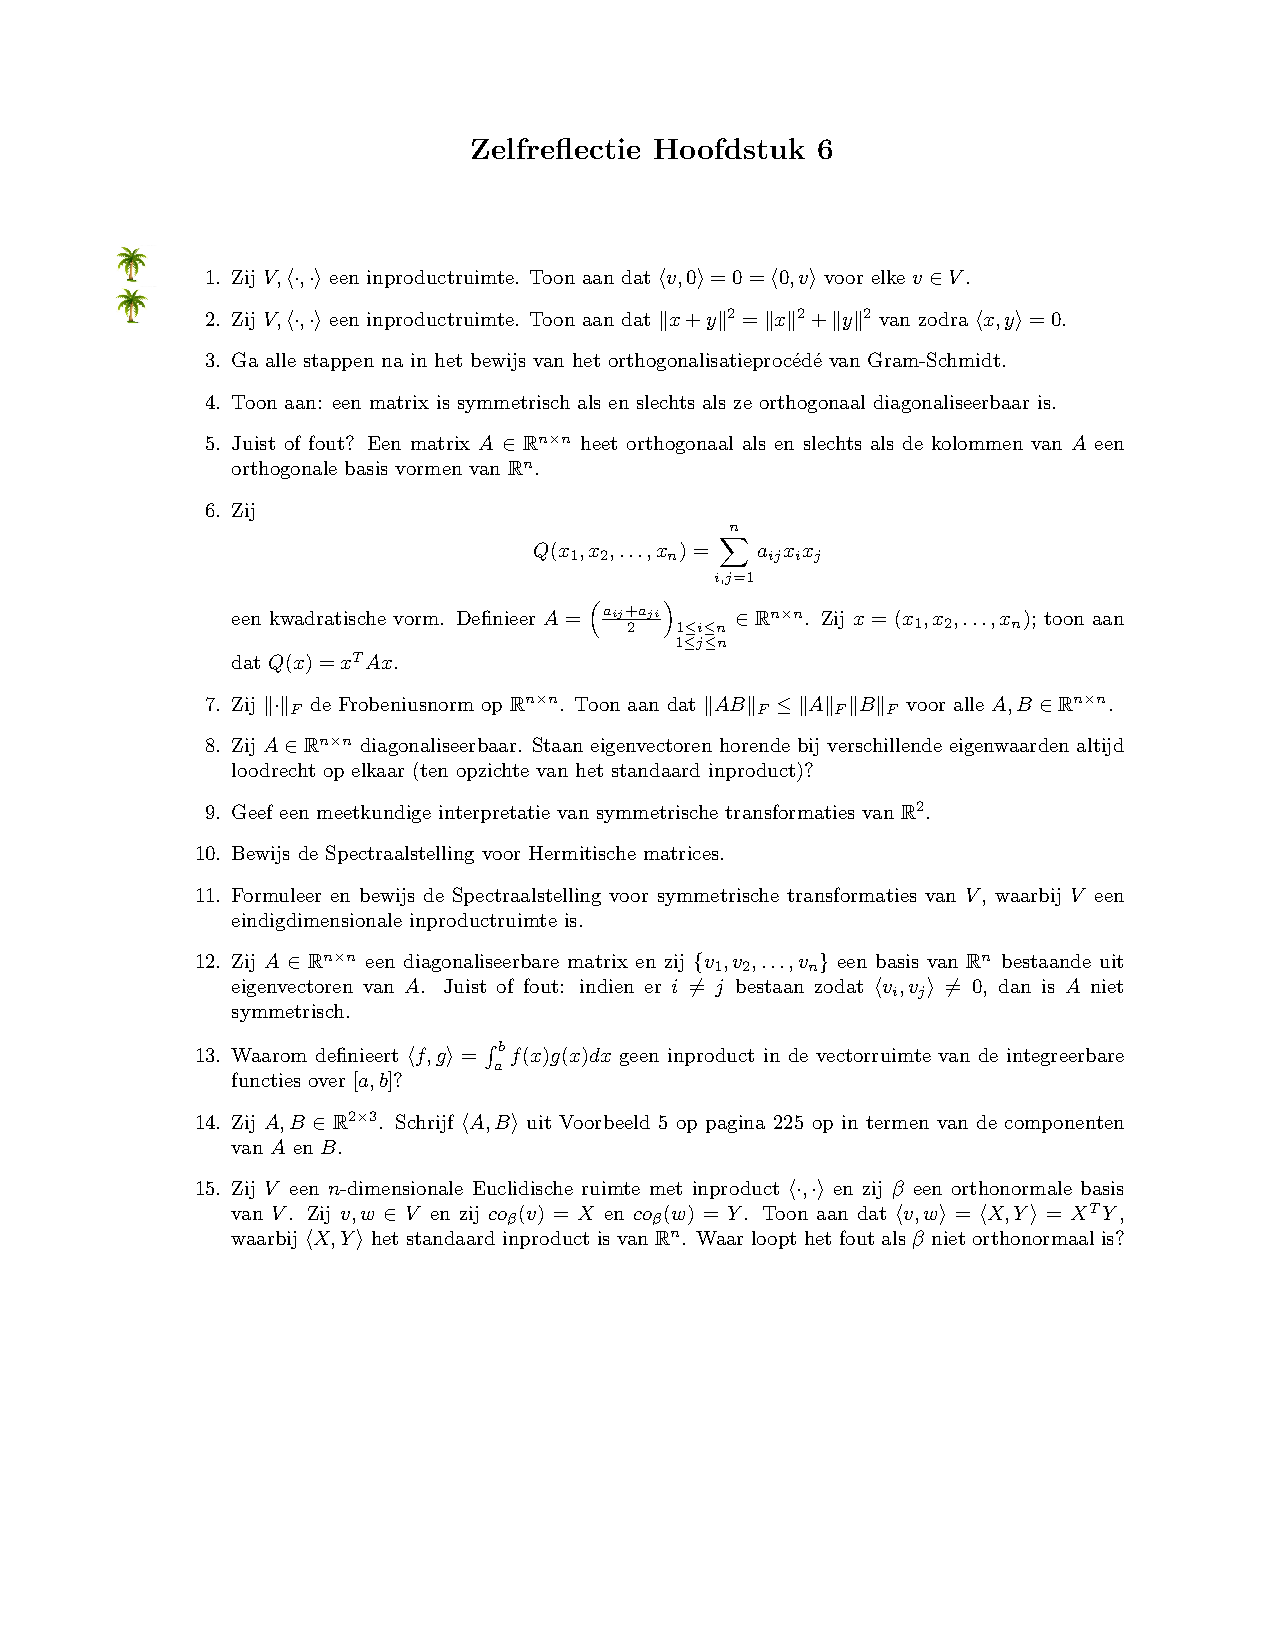
\includepdf[pages=-]{opgaven/zelfreflecties/zelfreflectie_H6.pdf}
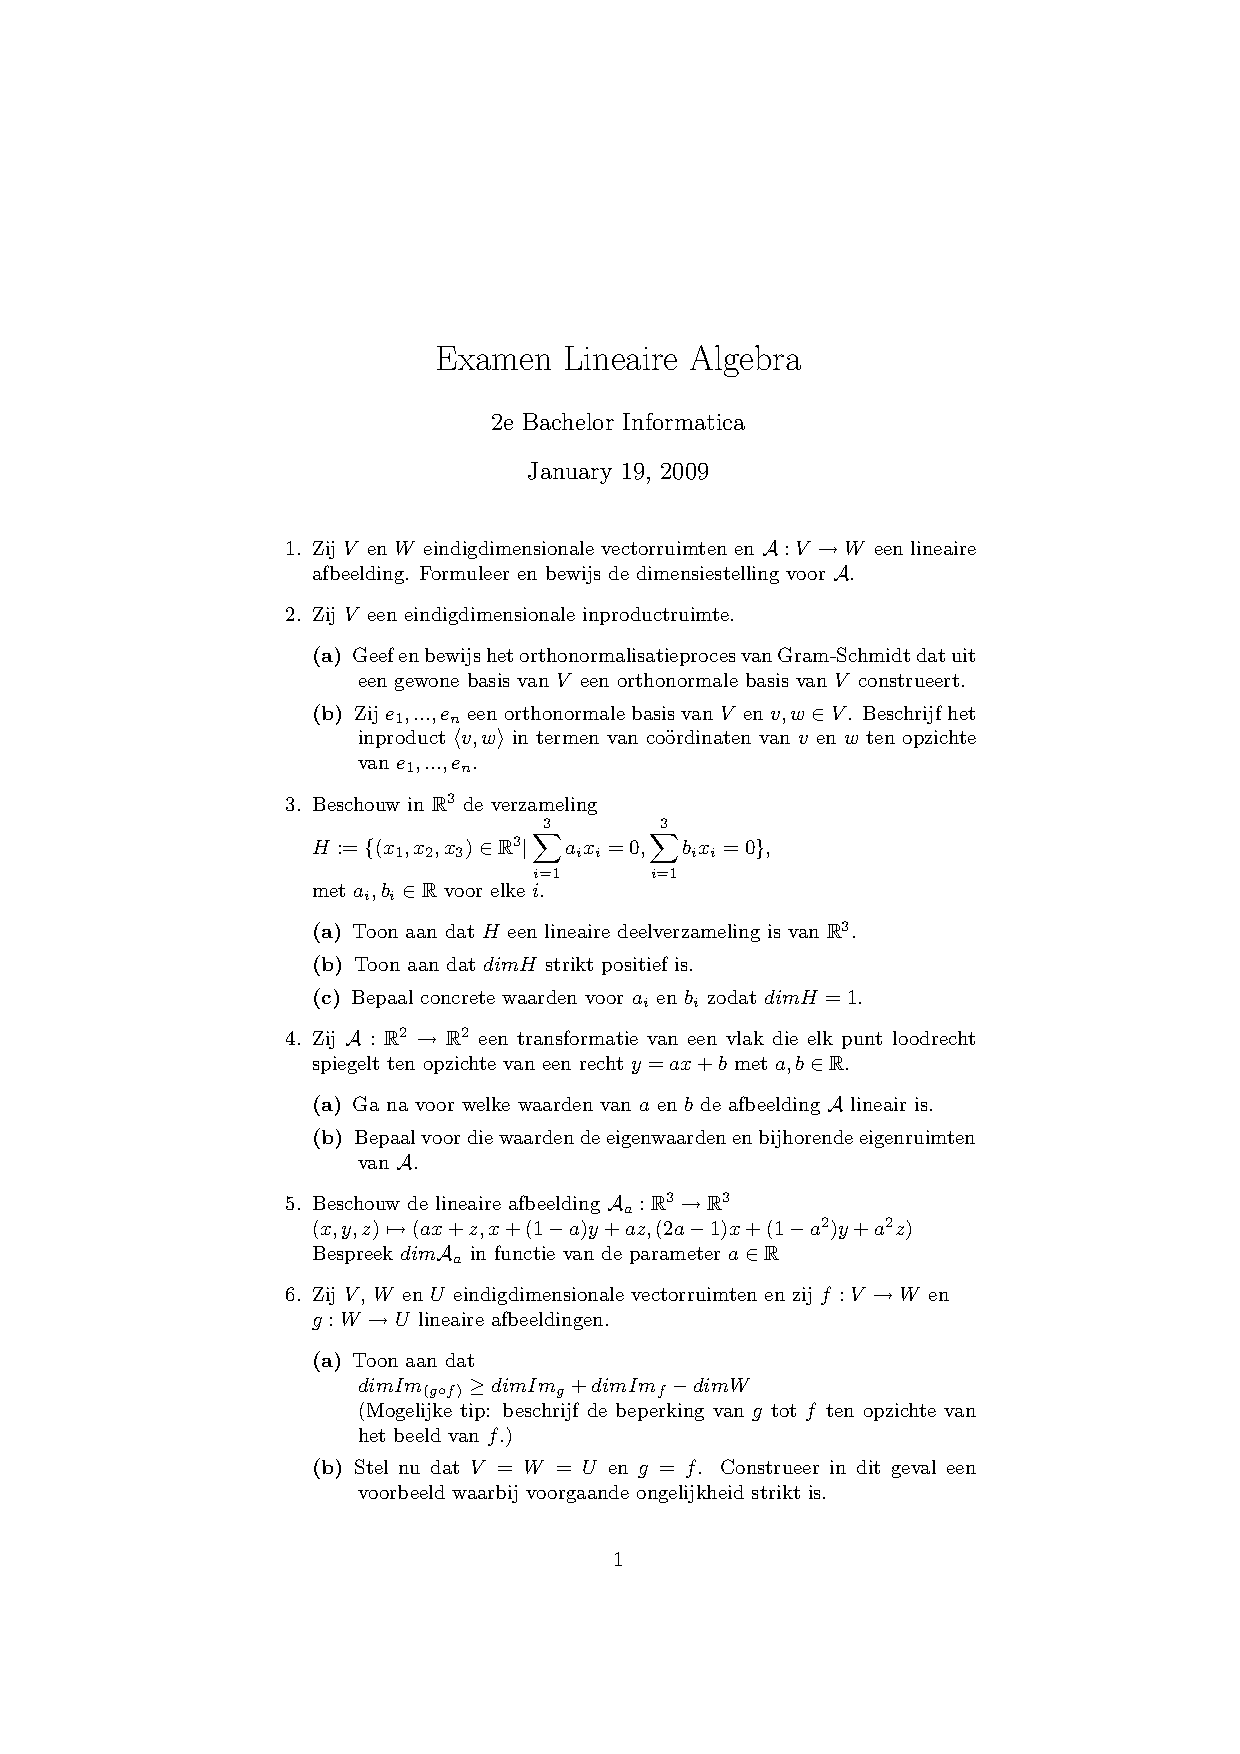
\includepdf[pages=-]{opgaven/examens/examen_2009_januari.pdf}
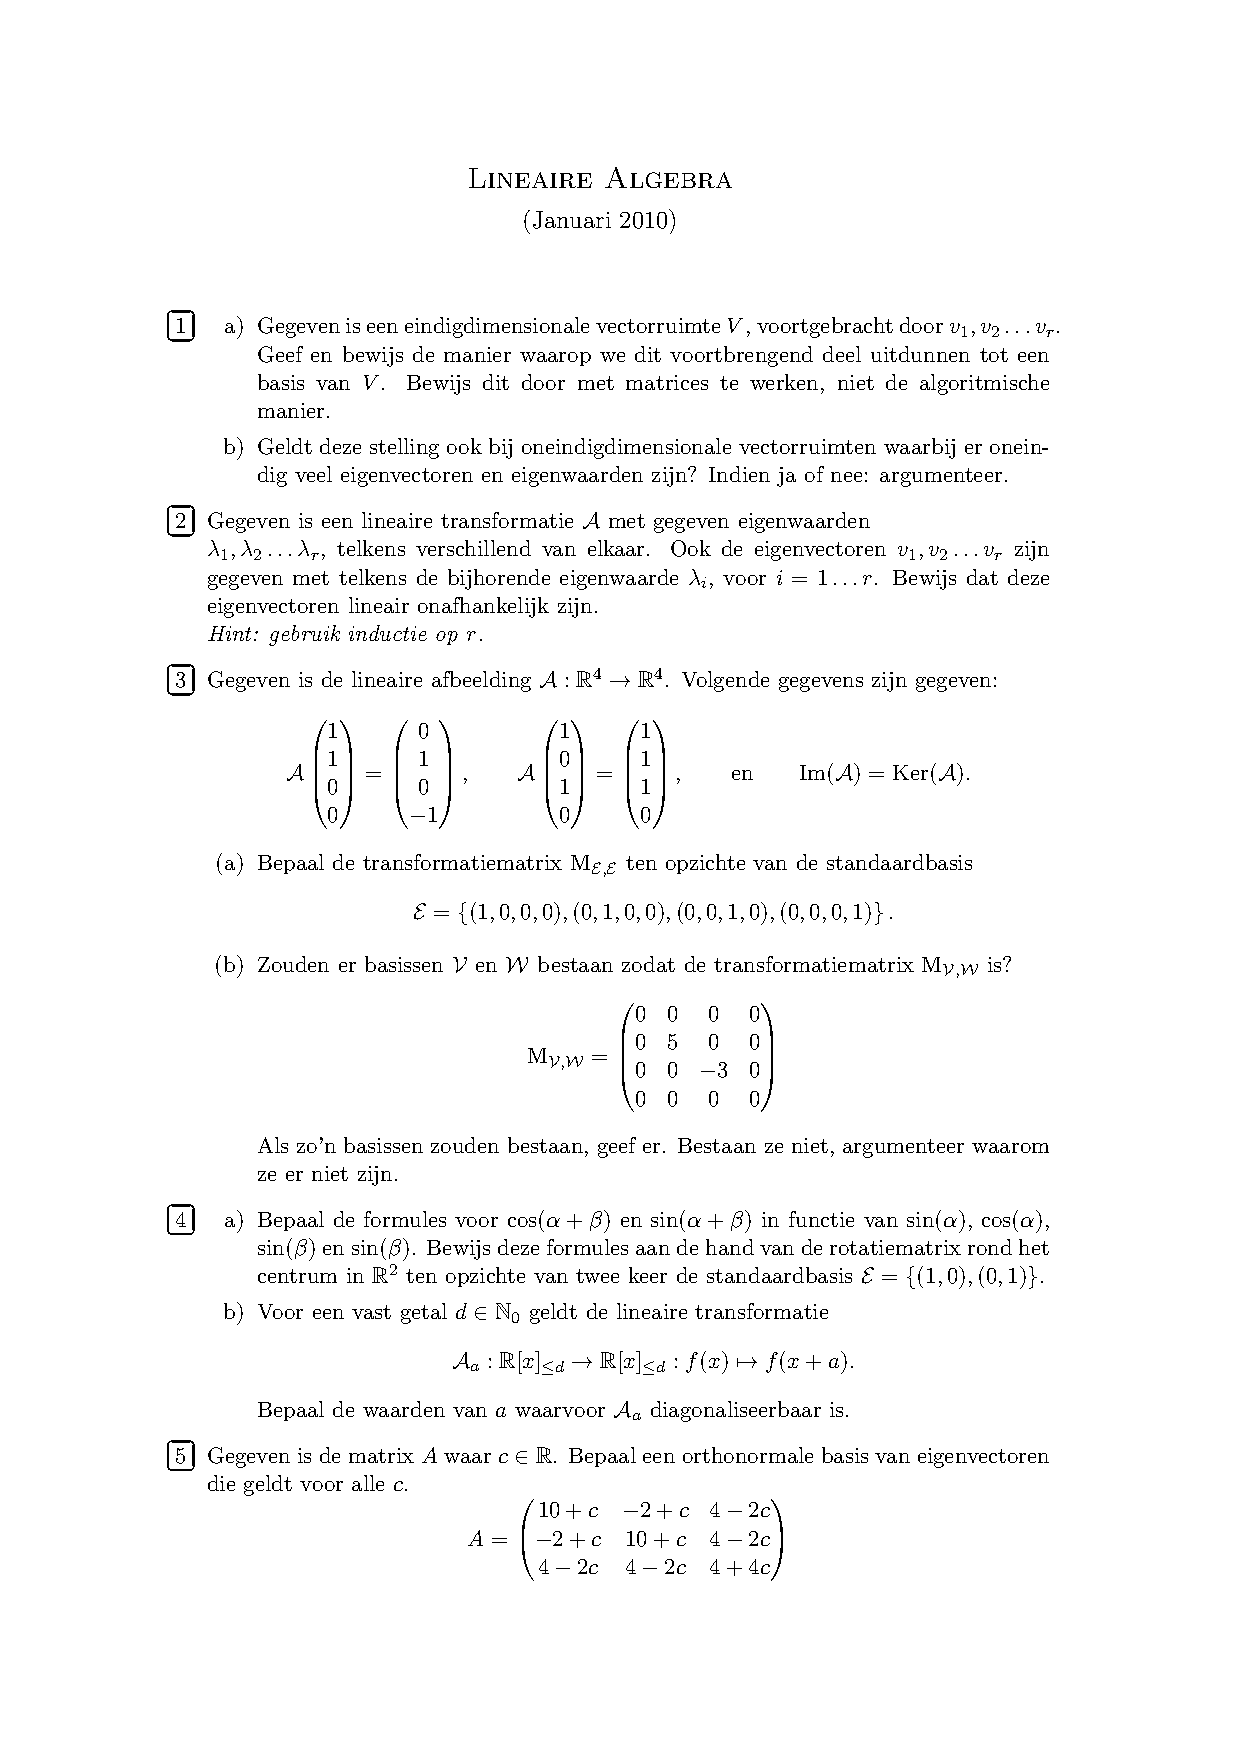
\includepdf[pages=-]{opgaven/examens/examen_2010_januari.pdf}
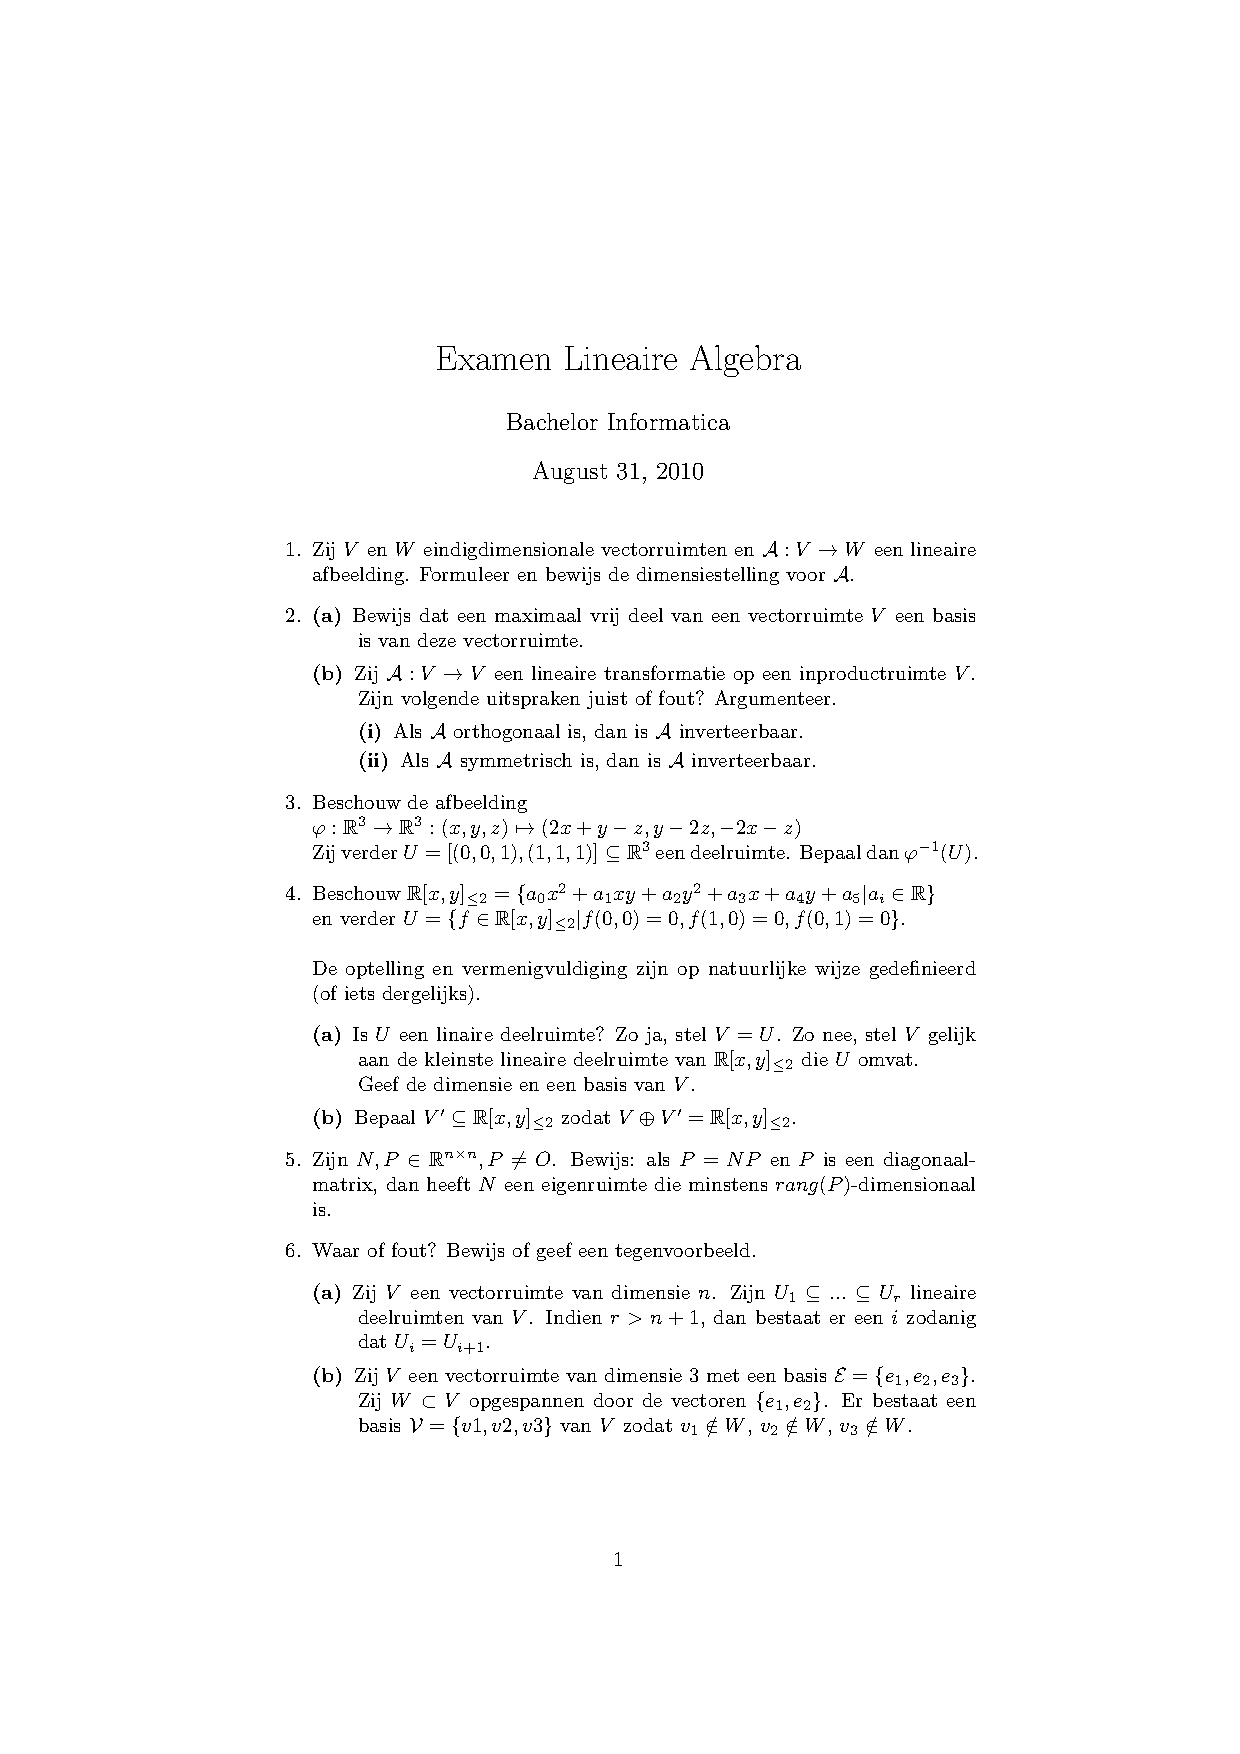
\includepdf[pages=-]{opgaven/examens/examen_2010_augustus.pdf}
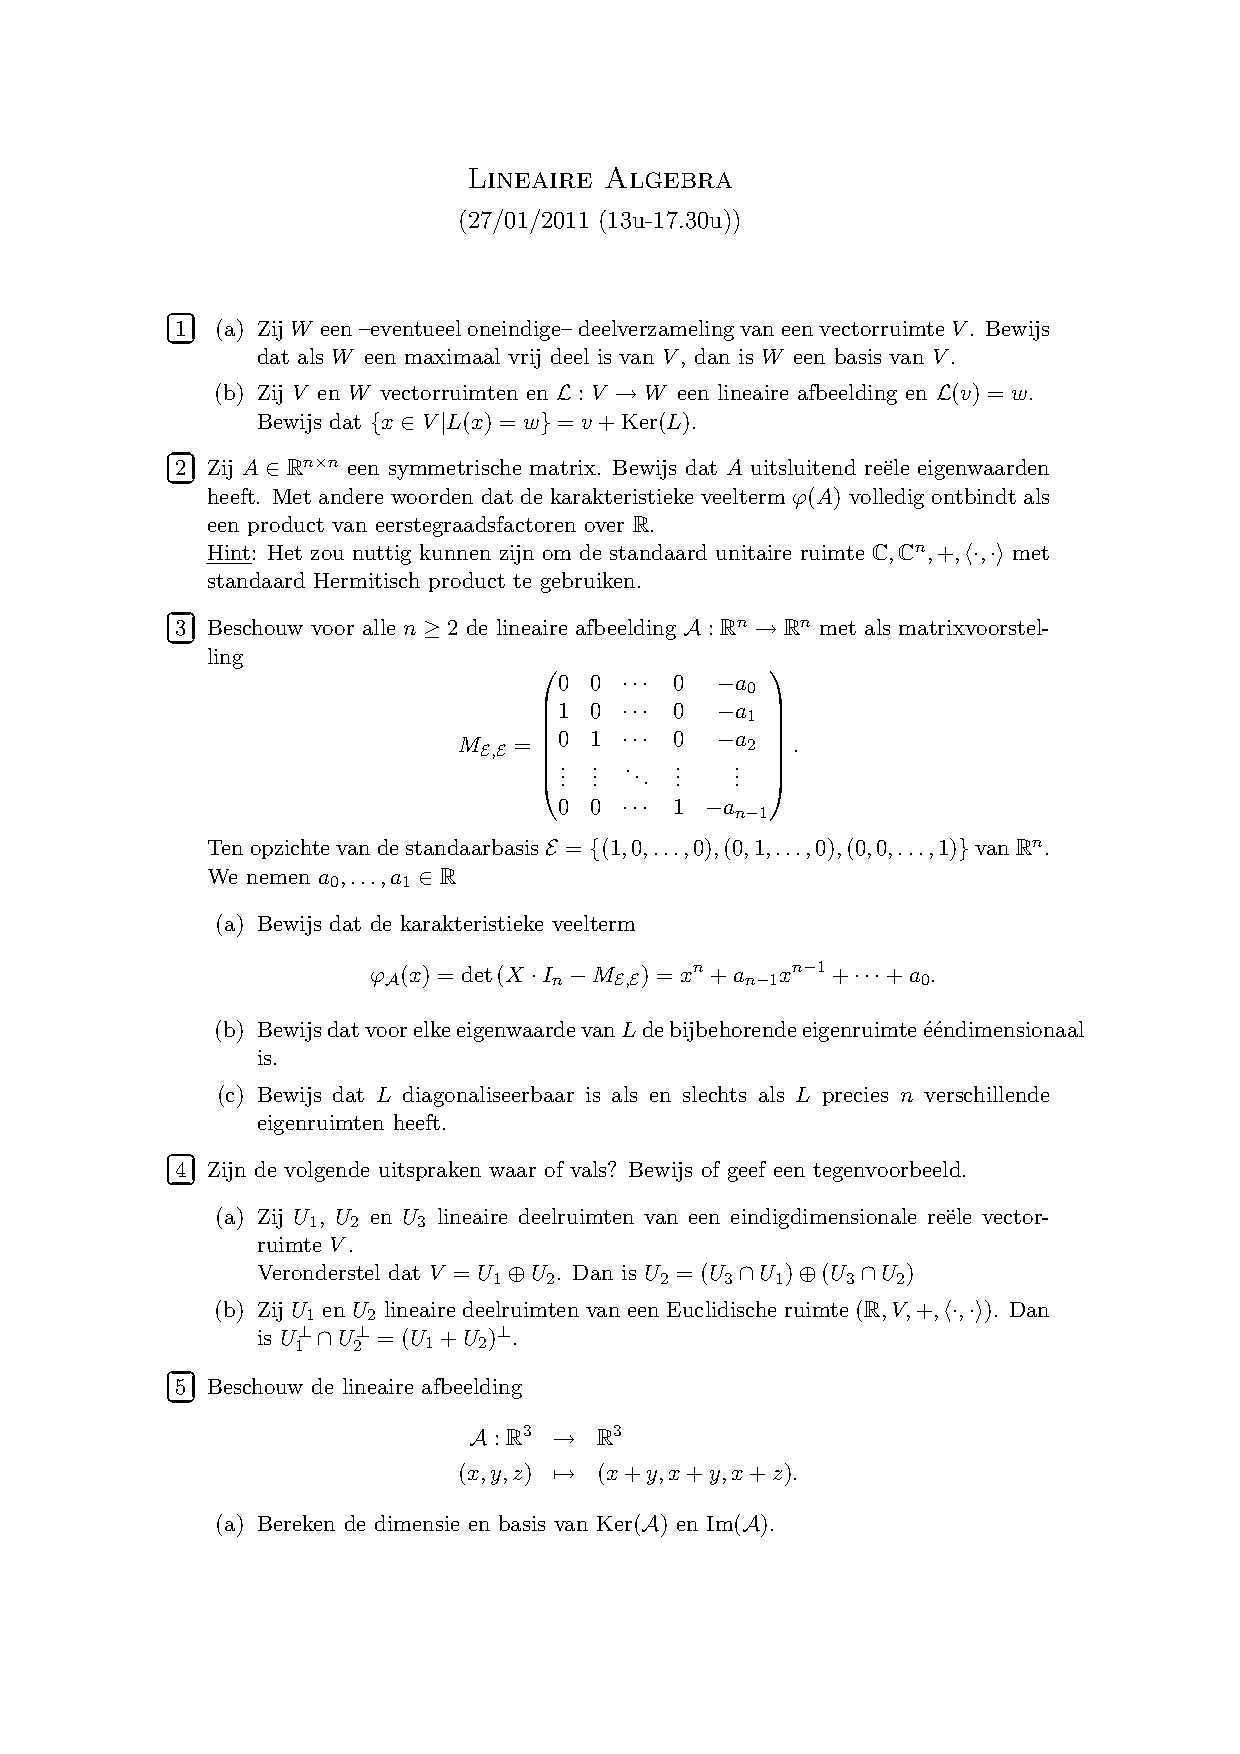
\includepdf[pages=-]{opgaven/examens/examen_2011_januari.pdf}
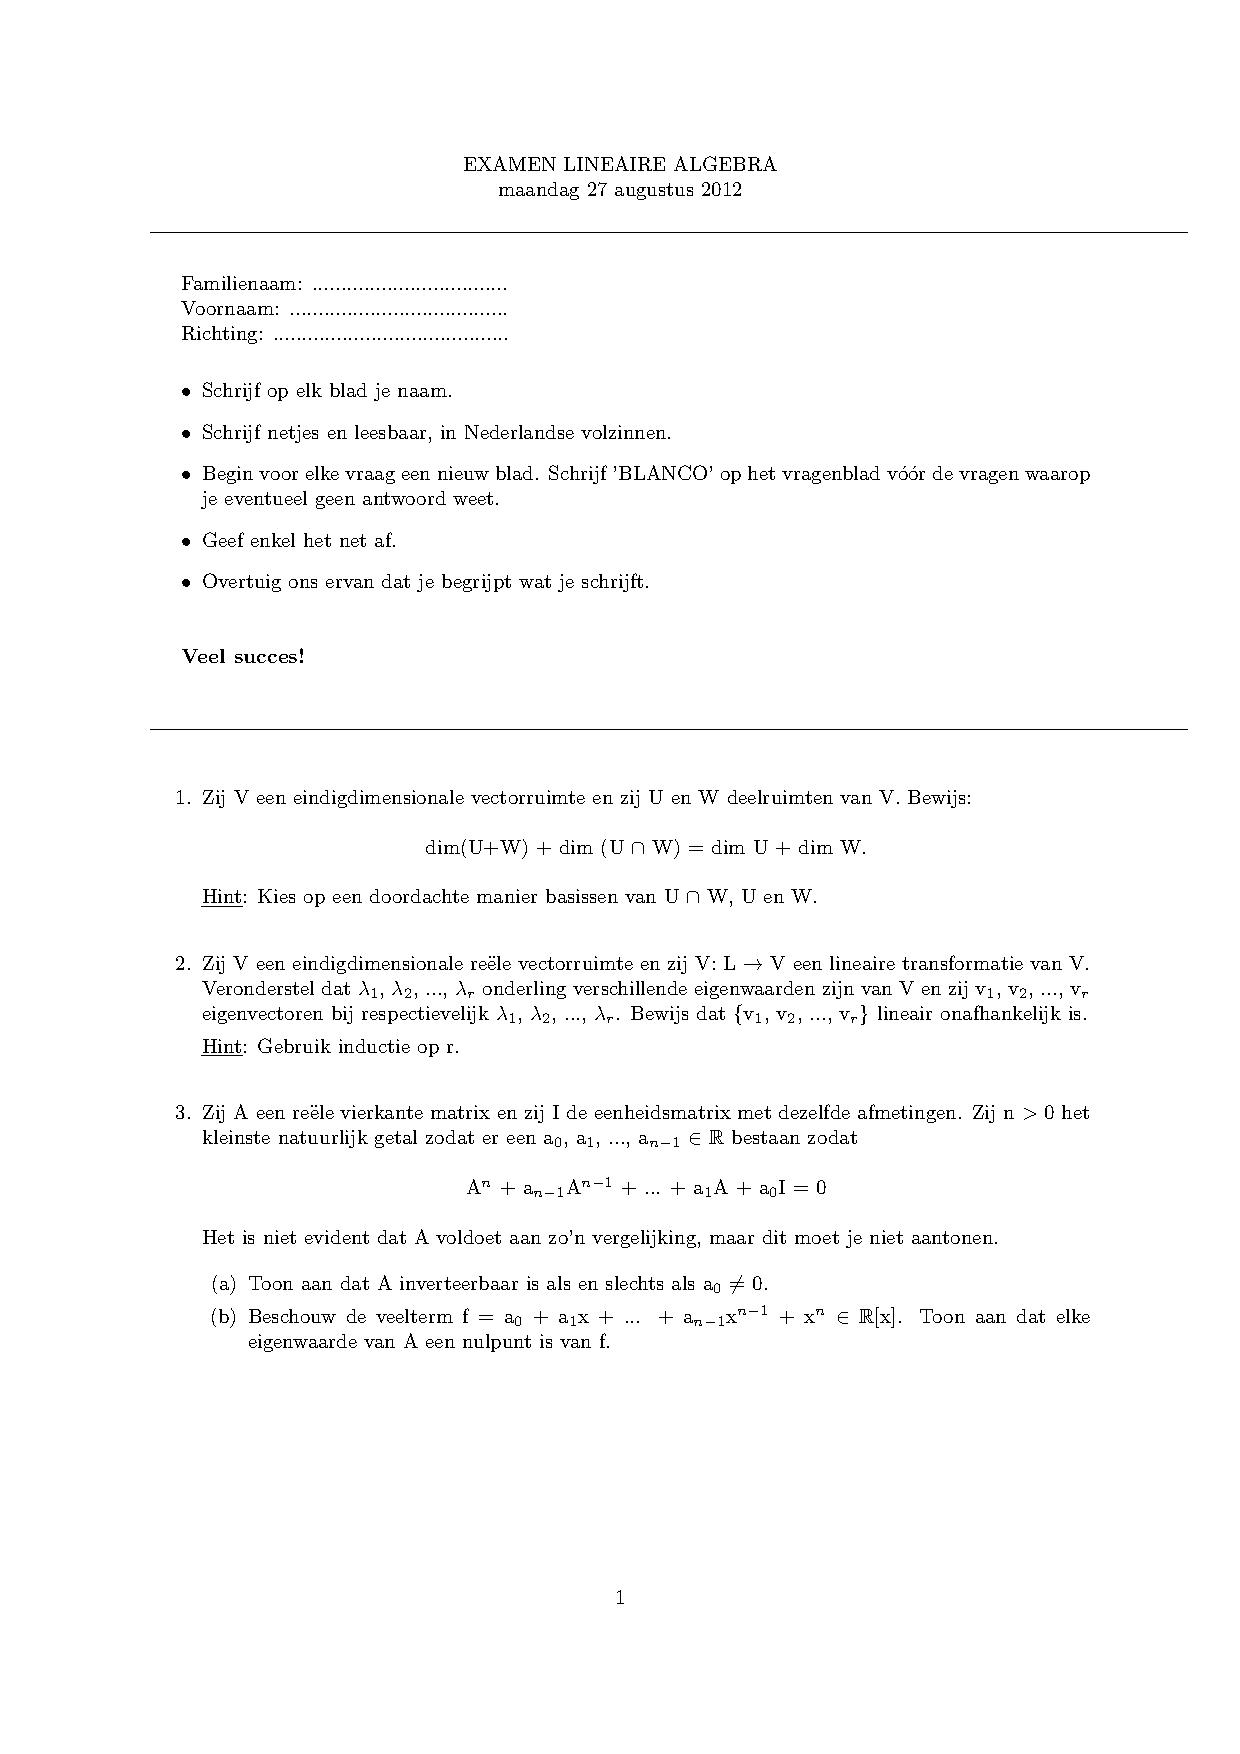
\includepdf[pages=-]{opgaven/examens/examen_2012_augustus.pdf}

\end{document}
